\chapter{Experimental methods}
\label{Chap2}

    In order to make the structure with the nanowires, we need to learn more about the different methods available in clean room. Moreover, we will make tests before starting with the nanowires that will help us to master the devices. I will describe here only the useful devices and methods for our process. In the last part, I talk about the dilution cryostats which I used to cool down some samples.
    
    \section{Resists}
        
        The resists are the central point of the fabrication, without them we would not be able to design the pattern we want and without pattern, no structure.
        
        \subsection{From theory...}
        
            The resists we use consists of polymer materials : Polymethyl Methacrilate (PMMA) (Fig. \ref{PMMA}) and Methyl Methacrilate (MMA).
            
            \begin{figure}[H]
            \centering
            \chemfig{CH_3-[:270]C(=[:180]CH_2)(-[:270]C(=[:0]O)(-[:270]O(-[:315]CH_3)))}
            \caption{Chemical structure of MMA, PMMA is a polymer made of this monomer}
            \label{PMMA}
            \end{figure}
            
            The resists are liquid, we depose them on the top of the wafer and then a spinner rotate the wafer and make a thin and uniform layer of resist.
            
            \begin{figure}[H]
                \centering
                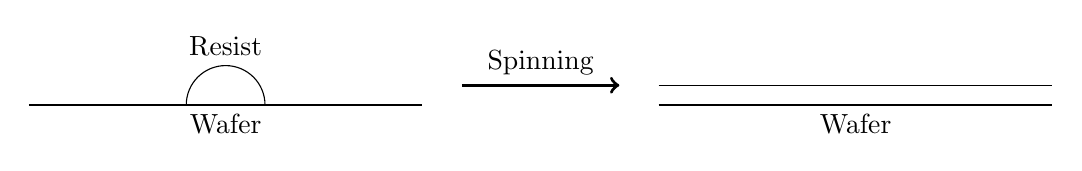
\begin{tikzpicture}
                    \draw [thick] (0,0)--(5,0);
                    \draw (3,0) arc(0:180:0.5);
                    \draw [->, very thick] (5.5,0.25)--(7.5,0.25)node[midway,above]{Spinning};
                    \draw [thick](8,0)--(13,0);
                    \draw (8,0.25)--(13,0.25);
                    \draw (2.5,0)node[below]{Wafer};
                    \draw (10.5,0)node[below]{Wafer};
                    \draw (2.5,0.5)node[above]{Resist};
                \end{tikzpicture}
                \caption{Spinner}
            \end{figure}
            
            The resists we use are sensitive to electrons, what we will do next is to send high energy electron onto them (See \ref{explicationebl}) which will imply structural modifications. The electron break the polymer into smaller pieces, which make the exposed resist more soluble in Methyl IsoButyl Ketone (MIBK) (See \ref{development}).
            
              Other type of resists exists, especially some resists damaged by light (photoresits), which are mostly used for semiconductors-based structures.
                          
        \subsection{...To practical}
        
            Practically, we use this two types of resists because they do not react the same way to exposure and development. First, we want a quite thick layer of MMA. Since the spinner create a fixed thickness, we repeat the proces until having the thickness we want, which means four times. Then we want a quite thin layer of PMMA, for this, only one spinning is good. When we have to bake the resists with a hot plate to make them solid instead of liquid. The resists have a data sheet where all necessary information is provided including optimal temperatures and baking durations. We finally obtain this (Fig. \ref{resine}) kind of cross-section view.
            
            \begin{figure}[H]
                \centering 
                \begin{tikzpicture}
                    \draw (0,0)--(10,0);
                    \draw (5,-0.5) node{Wafer $Si/SiO_2$};
                    \draw (0,2)--(10,2);
                    \draw (5,1)node{MMA};
                    \draw (0,2.5)--(10,2.5);
                    \draw (5,2.25) node{PMMA};
                \end{tikzpicture}
                \caption{Cross-section view after resist deposit, spinning and baking}
                \label{resine}
            \end{figure}
            
    \section{Electron Beam Lithography and development}
        
        Important part of the process, it determines either the structures will be as we expect or not, since it really impact the resist.
        
        \subsection{Electron Beam Lithography}
            The Electron Beam Lithographier (EBL) is a device which is used to design the patterns we want to have for our structures within the resist\cite{EBL_theory}. It sends a electron beam onto the resist to damage the bonds within it. The functionnal diagramm (Fig. \ref{EBLschema}) shows the ways the electrons are focused int the EBL. This diagram reminds some optical systems, since the goal is to focus eletrons on relatively small areas. Indeed, the size of the structures is quite small and we want to be the most accurate possible. This is why it is possible to adjust the resolution on the EBL, the accuracy of the beam. The higher the resolution is, the more time it takes to expose the resist, so the best thing is to find a compromise between resolution and time. For example, the only part that requires an good accuracy is the junction, so we have to use a good resolution there, but for the leads it does not matters much, so we choose to go faster. Then, the other adjustable parameter is the exposure dose, which means the amount of electron we send through the resist. The higher the exposure dose is, the more it damages the resist. As for the resolution, we have to find a compromise between enough electrons to make sure the bonds are destroyed within the resist and avoid completely burning it. 
            The EBL is designed to send electron onto the resist, yet, these electrons have a too high energy to break the bonds of polymers. Actually, when they encounter matter, they generate other electrons from atoms, named secondary electrons. These are these eletrons who have the right energy to break the bonds of polymers. The goal of the EBL is to generate the larger amount of secondary electrons possible and this is achieved by using high energy incident electrons that can penetrate deeply within the resist layer. The deeper they go, the more secondary electrons they generate and more bond are broken.

            \label{explicationebl}
            
            \begin{figure}[H]
                    \centering
                    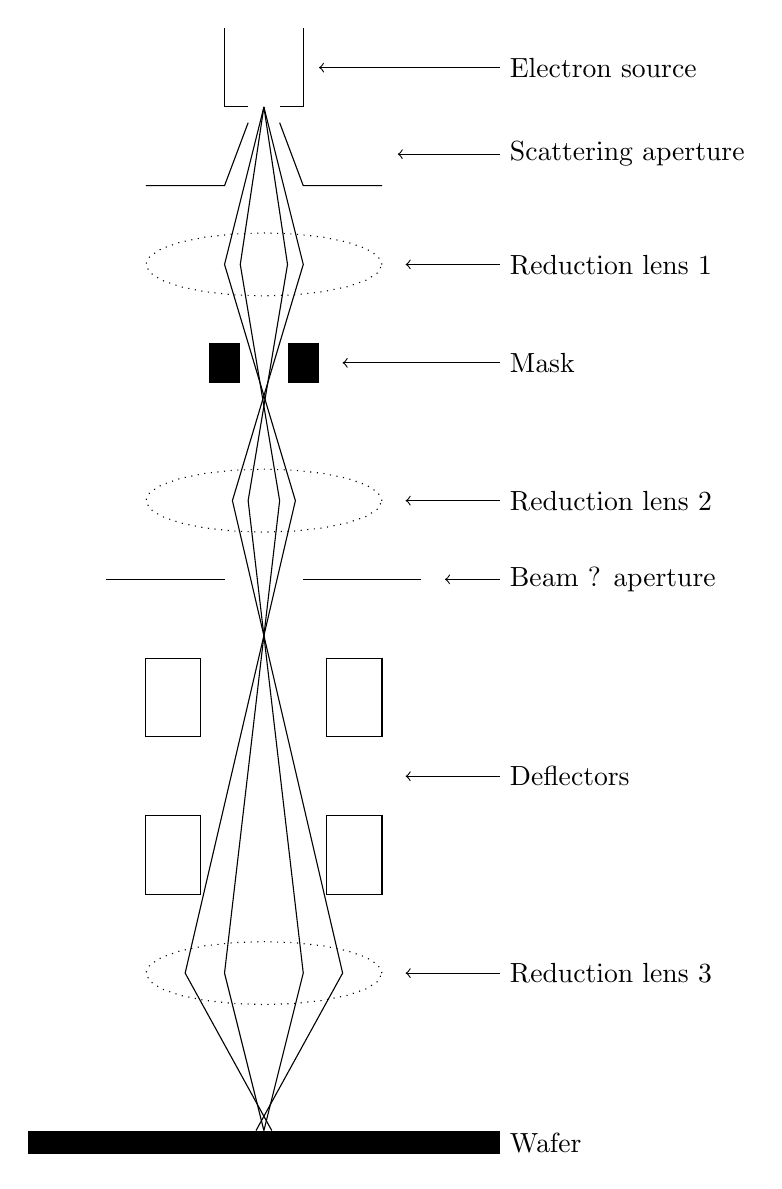
\begin{tikzpicture}
                    \draw (4.5,20)--(4.5,19)--(4.8,19);
                    \draw (5.2,19)--(5.5,19)--(5.5,20);
                    \draw [<-] (5.7,19.5)--(8,19.5);
                    \draw (8,19.5)node[right]{Electron source};
                    
                    \draw (3.5,18)--(4.5,18)--(4.8,18.8);
                    \draw (6.5,18)--(5.5,18)--(5.2,18.8);
                    \draw [<-] (6.7,18.4)--(8,18.4);
                    \draw (8,18.4)node[right]{Scattering aperture};
                    
                    \draw [dotted] [domain=0:360] plot({1.5*cos(\x)+5},{0.4*sin(\x)+17)});
                    \draw [<-] (6.8,17)--(8,17);
                    \draw (8,17)node[right]{Reduction lens 1};
                    
                    \fill (4.7,16)--(4.7,15.5)--(4.3,15.5)--(4.3,16)--cycle;
                    \fill (5.3,16)--(5.3,15.5)--(5.7,15.5)--(5.7,16)--cycle;
                    \draw [<-] (6,15.75)--(8,15.75);
                    \draw (8,15.75)node[right]{Mask};
                    
                    \draw [dotted] [domain=0:360] plot({1.5*cos(\x)+5},{0.4*sin(\x)+14)});
                    \draw [<-] (6.8,14)--(8,14);
                    \draw (8,14)node[right]{Reduction lens 2};
                    
                    \draw (3,13)--(4.5,13);
                    \draw (7,13)--(5.5,13);
                    \draw [<-] (7.3,13)--(8,13);
                    \draw (8,13) node[right]{Beam ? aperture};
                    
                    \draw (3.5,12)--(4.2,12)--(4.2,11)--(3.5,11)--cycle;
                    \draw (6.5,12)--(5.8,12)--(5.8,11)--(6.5,11)--cycle;
                    \draw (3.5,10)--(4.2,10)--(4.2,9)--(3.5,9)--cycle;
                    \draw (6.5,10)--(5.8,10)--(5.8,9)--(6.5,9)--cycle;
                    \draw [<-](6.8,10.5)--(8,10.5);
                    \draw (8,10.5)node[right]{Deflectors};
                                                            
                    \draw [dotted] [domain=0:360] plot({1.5*cos(\x)+5},{0.4*sin(\x)+8)});
                    \draw [<-] (6.8,8)--(8,8);
                    \draw (8,8)node[right]{Reduction lens 3};
                    
                    \fill (2,6)--(8,6)--(8,5.7)--(2,5.7)--cycle;
                    \draw (8,5.85) node[right]{Wafer};
                    
                    \draw (5,19)--(4.5,17)--(5.4,14)--(4,8)--(5.1,6);
                    \draw (5,19)--(5.5,17)--(4.6,14)--(6,8)--(4.9,6);
                    \draw (5,19)--(4.7,17)--(5.2,14)--(4.5,8)--(5,6);
                    \draw (5,19)--(5.3,17)--(4.8,14)--(5.5,8)--(5,6);
                    \end{tikzpicture}
                    \caption{Simplified EBL functional diagram}
                    \label{EBLschema}
            \end{figure}
            
            \begin{figure}[H]
                \centering
                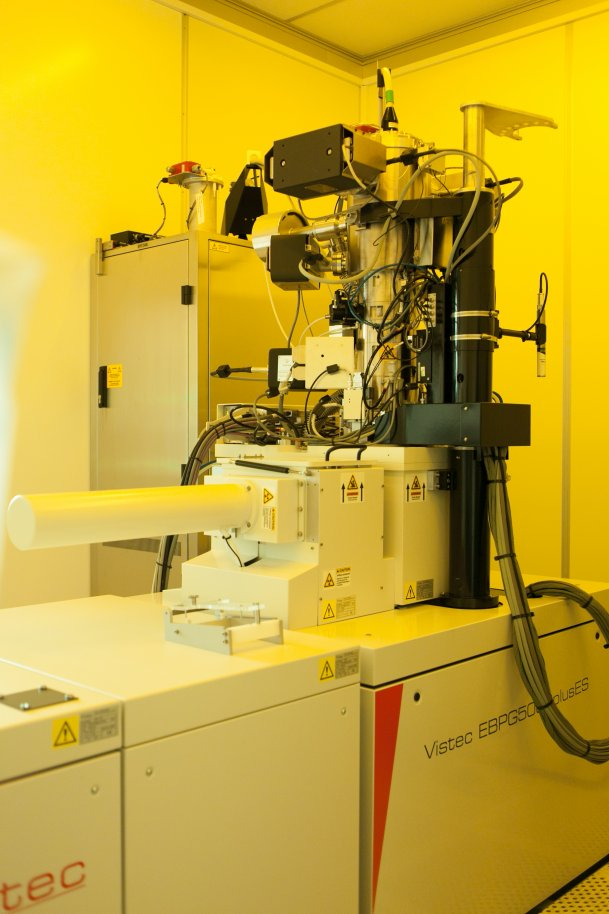
\includegraphics[width=100pt]{EBL.jpg}
                \caption{Electron Beam Lithographier Vistec of Micronova clean room}
            \end{figure}
            
        \subsection{Pattern design}
        
            The beam is controled by computers, we can create all the designs we want in a software and import them to make the EBL expose the resist. The beam breaks the bonds in the selected zones, as show the Fig. \ref{waferEBL}.
            
            \begin{figure}[H]
                \centering
                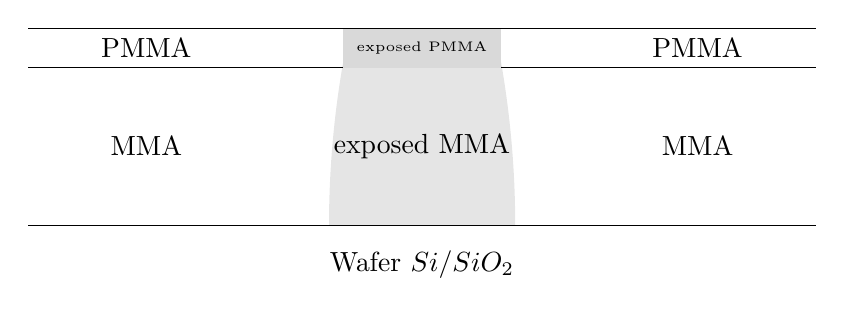
\begin{tikzpicture}
                \draw (5,-0.5) node{Wafer $Si/SiO_2$};
                \fill [color=gray!20] (3.82,0) arc(180:170:12)--++(2,0) arc (10:0:12)--cycle;
                \draw (0,2)--(4,2);
                \draw (6,2)--(10,2);
                \draw (1.5,1) node{MMA};
                \draw (8.5,1) node{MMA};
                \draw (1.5,2.25) node{PMMA};
                \draw (8.5,2.25) node{PMMA};
                \fill [color=gray!30] (4,2)--(4,2.5)--(6,2.5)--(6,2)--cycle;
                \draw (0,2.5)--(10,2.5);
                \draw (5,2.25)node{{\tiny exposed PMMA}};
                 \draw (0,0)--(10,0);
                \draw (5,1)node{exposed MMA};
                \end{tikzpicture}
                \caption{Cross-section view after EBL}
                \label{waferEBL}
            \end{figure}
        
        \subsection{Development}
            \label{development}
            Development consists in the withdrawal of the exposed resit. It is realized by a succession of chemical reactions. First of all, we have to pierce the PMMA to access the MMA. It is the role of MIBK (Fig. \ref{MIBK}) to dissolve the exposed PMMA and MMA. The MIBK pierces a strait hole in the resist (Fig. \ref{aprèsMIBK}), but it will not be enough for the structures we want to do. Our goal is to make small junction between Al and Cu, if we depose Al or Cu on this wafer, 
                       
            \begin{figure}[H]
                \centering
                \chemfig{-[:-30](-[:30]-[:-30](-[:30])(=[:270]O))(-[:270])}
                \caption{Chemical structure of MethylIsoButylKetone (MIBK)}
                \label{MIBK}
            \end{figure}
Our goal is to make small junction between Al and Cu, if we depose Al or Cu on this wafer, they will depose everywhere and we will just have Aluminium covered by Copper, which is not what we want. To manage to make the structure, you have to find a way to not depose metal everywhere. This is the role of the undercuts ans evaporation angles (See \ref{evapangles}). We add a step to the development : we dive the chip in MethyGlycol. MethyGlycol can dissolve MMA even if this one have not been exposed to the electron beam, but do not damage PMMA. This allows us to create a dome, a larger empty area below the PMMA (Fig. \ref{Aprèsdvpt}) named undercut. There, we can see that if we depose metal along a certain angle, they will not necessarily be in contact, this is what we are looking for. The final step of development is to stop the reaction. We dive the sample in Isopropanol which is neutral with our two resist and stops the reaction with MethyGlycol.
Of course, the reactions follow some kind of kinetics and the dissolution will depend on the time we dive the samples into the chemicals. Indeed, electron exposure only ease the dissolution of the resists, this means that we cannot just let the dissolution go and come back when it is over, we have to determine the accurate duration for our application. If it is less important for MIBK (because the difference between dissolution coefficients of exposed and non-exposed resist is large enough), it is very important for MethyGlycol. We have to make sure the undercuts are large enouch for our structures but ensure that PMMA does not collapse.
            
            \begin{figure}[H]
                \centering
                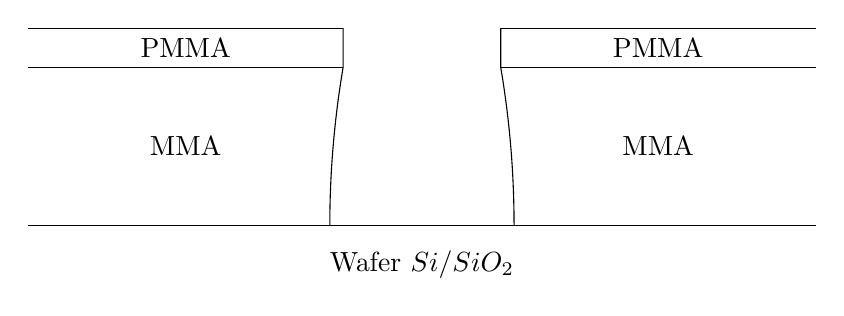
\begin{tikzpicture}
                \draw (5,-0.5) node{Wafer $Si/SiO_2$};
                \draw (3.83,0) arc(180:170.4:12)--++(0,0.5);
                \draw (6.17,0) arc(0:9.6:12)--++(0,0.5);
                \draw (0,2)--(4,2);
                \draw (6,2)--(10,2);
                \draw (0,2.5)--(4,2.5);
                \draw (6,2.5)--(10,2.5);
                \draw (0,0)--(10,0);
                \draw (2,1)node{MMA};
                \draw (8,1)node{MMA};
                \draw (8,2.25)node{PMMA};
                \draw (2,2.25)node{PMMA};
                \end{tikzpicture}
                \caption{Cross-section view after MIBK}
                \label{aprèsMIBK}
            \end{figure}
            

            \begin{figure}[H]
            \centering
            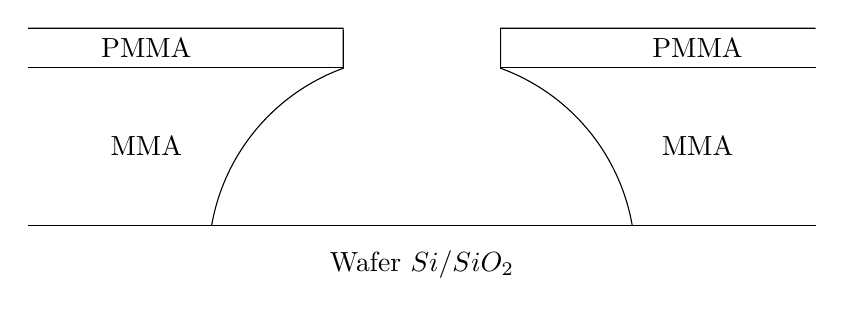
\begin{tikzpicture}
                \draw (0,0)--(10,0);
                \draw (5,-0.5) node{Wafer $Si/SiO_2$};
                \draw (2.33,0) arc(170:110:2.6)--(4,2.5)--(0,2.5);
                \draw (7.67,0) arc(10:70:2.6)--(6,2.5)--(10,2.5);
                \draw (0,2)--(4,2);
                \draw (6,2)--(10,2);
                \draw (1.5,1) node{MMA};
                \draw (8.5,1) node{MMA};
                \draw (1.5,2.25) node{PMMA};
                \draw (8.5,2.25) node{PMMA};
            
            \end{tikzpicture} 
            \caption{Cross-section after full development}
            \label{Aprèsdvpt}
            \end{figure}
            
    \section{Evaporator}
        The main part of the process, where we actually make the structures by evaporating metal.
        \subsection{Functioning of evaporator}
        
        The evaporator is a tool that allows to deposit a uniform, thin layer of metal inside the undercuts newly developped. A filament is submitted to a huge tension and current, it emits photons that will melt the metal and tear atoms from it. These atoms can move freely in the very low pressure chamber ($P\sim10^{-7}mbar$) : the mean free path is long enough to allows atoms to go everywhere in the chamber especially in our undercuts. The deposition of the atoms is very uniform and there are sensors to measure the thickness of the layer. So, we can set the thickness we want and the device will automatically stop when the thickness reaches this value.
        There is a valve for Oxygen, so that we can oxidize. It is partiularly helpful to realize insulators \textit{in situ}, Al$_2$Ox$_3$ is an insulator and it create an energy barrier, quantically speaking.
        There is also a Plasma Gun, with Argon valve. The plasma is mostly used to ease the lift-off (See \ref{lift-off}) by weakening the resist. But with the accurate parameters it can also tear atoms for samples, this is a technique called plasma etching, and we will use it quite a lot. The second goal of this project is to characterize this technique in the evaporator here : characterize the plasma and determine its effect on samples (See \ref{Chap3}). We need to know better about plasma etching because the nanowires will come from Copenhaguen and the Aluminium layer will be strongly oxidized, thing that we do not want. We will need to get rid of it one way or another, this is why we try plasma etching.           
            
            \begin{figure}[H]
                \centering
                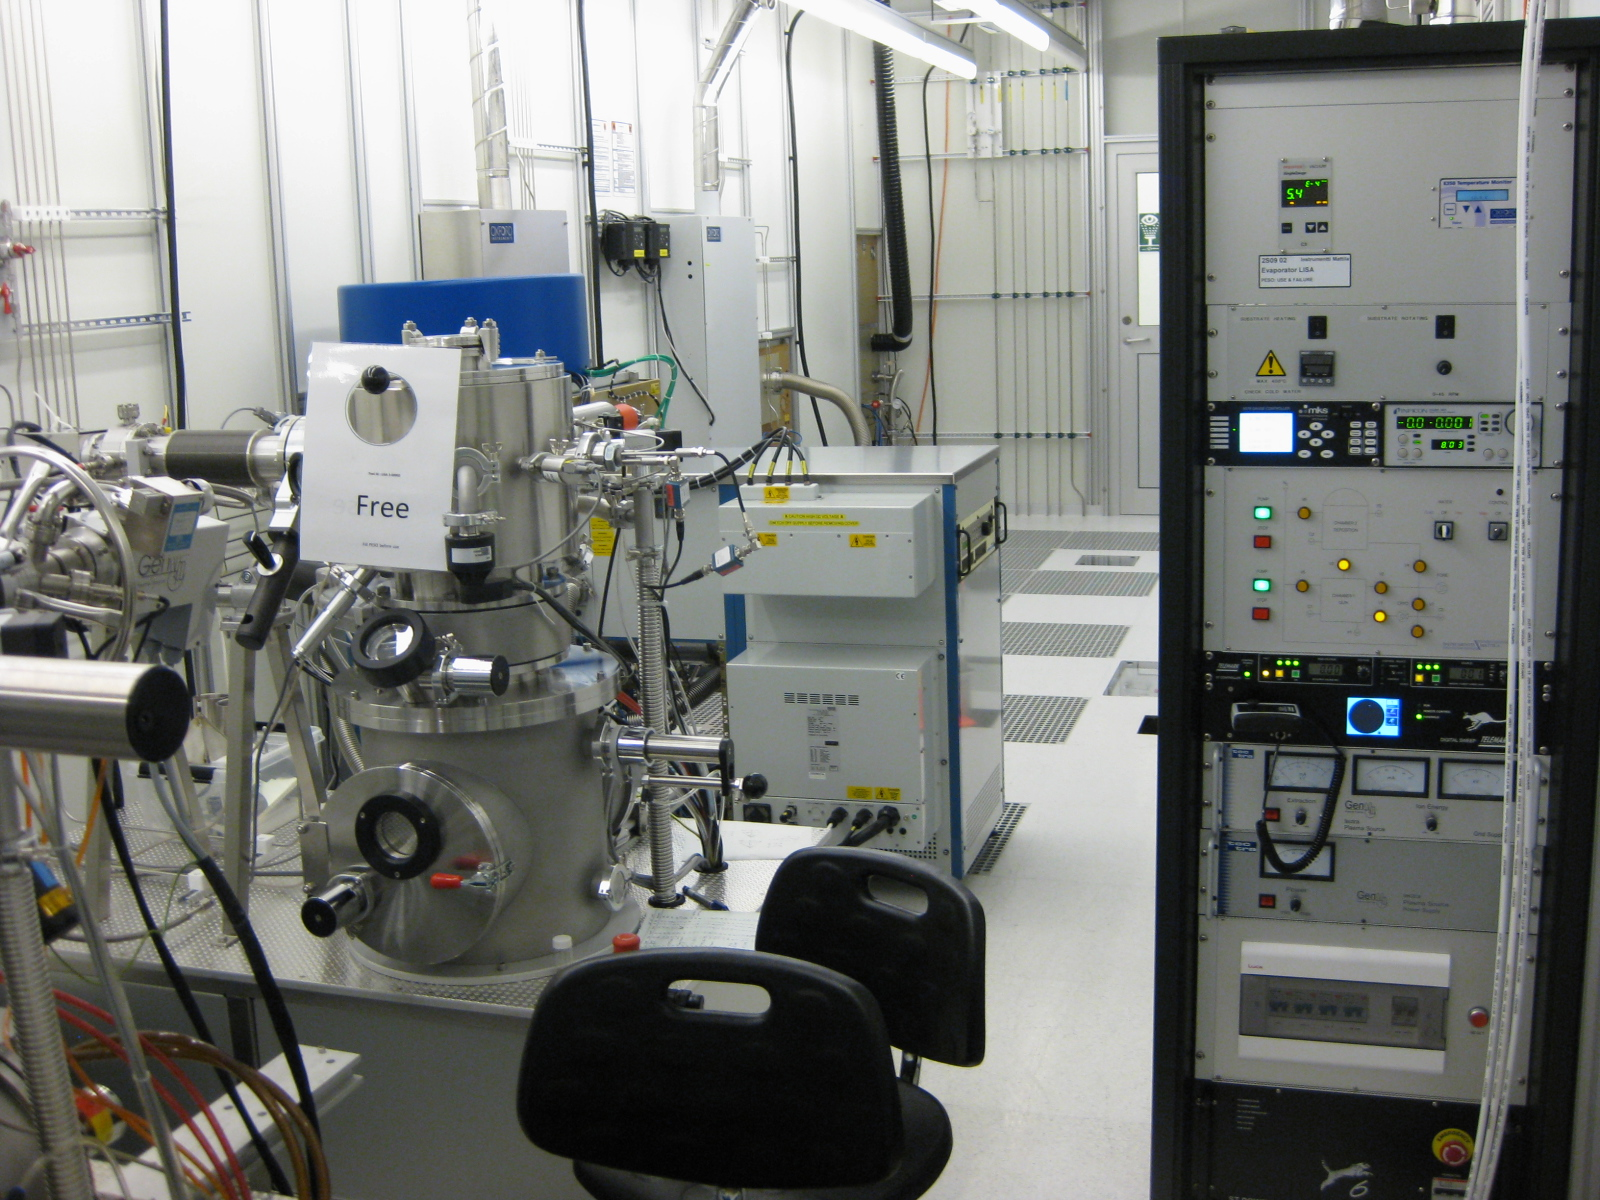
\includegraphics[width=200pt]{LISA.JPG}
                \caption{Photographie de l'évaporateur LISA utilisé pour réaliser les structures}
            \end{figure}
            
            
            \subsection{Evaporator in action}
            
                \label{evapangles}
                The Fig. \ref{evaporation} shows what happens in the evaporation chamber. First, we depose Aluminium with a previously determined angle, then the evaporate Copper, with another angle. Thus, we can see that even it they are in the same undercut, they do not touch each other. To make the junction, we have to have two different undercut that overlap. Like this it is the metal from one undercut which will be in contact with the other metal for the other undercut so that they are in contact in a tiny area and not in the whole pattern. Of course, we can add others steps to this processe like oxidation and plasma.
                
            \begin{figure}[H]
            \centering
            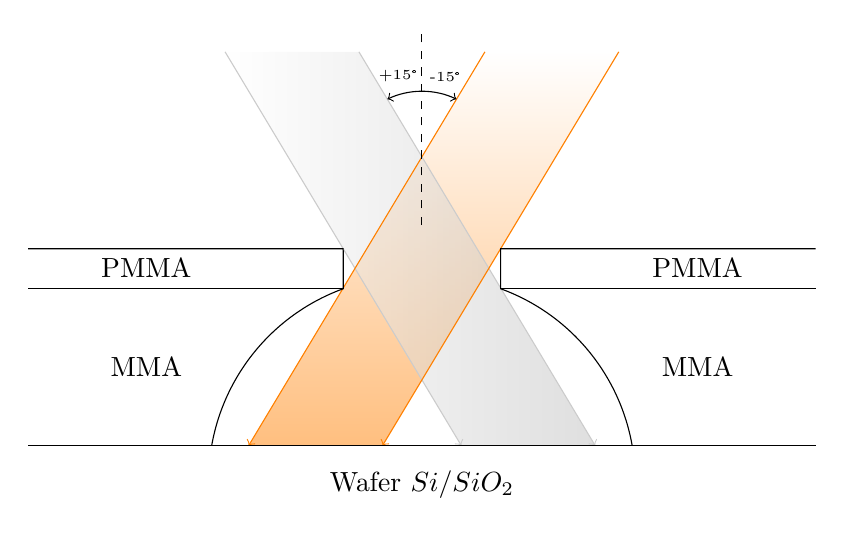
\begin{tikzpicture}
                
                \shadedraw[bottom color=orange,top color=white, draw=orange, fill opacity=0.5,draw opacity=0](5.8,5)--(2.8,0)--(4.5,0)--(7.5,5)-- cycle;
                \shadedraw[right color=gray!50,left color=white, draw=gray!40, fill opacity=0.5, draw opacity=0](4.2,5)--(7.2,0)--(5.5,0)--(2.5,5)--cycle;   
                \draw [color=gray!40,->] (4.2,5)--(7.2,0);
                \draw [color=gray!40,->] (2.5,5)--(5.5,0);  
                \draw [color=orange,->] (5.8,5)--(2.8,0);
                \draw [color=orange,<-] (4.5,0)--(7.5,5);
                          
                \draw (0,0)--(10,0);
                \draw (5,-0.5) node{Wafer $Si/SiO_2$};
                \draw (2.33,0) arc(170:110:2.6)--(4,2.5)--(0,2.5);
                \draw (7.67,0) arc(10:70:2.6)--(6,2.5)--(10,2.5);
                \draw (0,2)--(4,2);
                \draw (6,2)--(10,2);
                \draw (1.5,1) node{MMA};
                \draw (8.5,1) node{MMA};
                \draw (1.5,2.25) node{PMMA};
                \draw (8.5,2.25) node{PMMA};
                \draw [dashed](5,2.8)--(5,5.3);
                \draw [->] (5,4.5) arc(90:116:1);
                \draw (4.7,4.5)node[above]{{\tiny +15\textdegree}};
                \draw [->] (5,4.5) arc(90:64:1);
                \draw (5.3,4.5)node[above]{{\tiny -15\textdegree}};
                
            \end{tikzpicture} 
            \caption{Cross-section during evaporation}
            \label{evaporation}
            \end{figure}
                
                
                
    \section{Lift-off and Scanning Electron Microscope}
        Final part of the process where we complete the structures and check if everything was fine.
        \subsection{Lift-off : resist withdrawal}
        \label{lift-off}
        
            Metals evaporated everywhere on the chip but, they mainly are upon the resist. The structures are protected inside the undercuts. So, we will just dissolve the resist with aceton. It will take the metal off the wafer and let only the structures.
            
        \subsection{Scanning Electron Microscope functioning}
            The functioning of Scanning Electron Microscope (SEM) is very similar to the EBL one, since actually, SEM can be used as EBL, except that this time we do not want to weaken the matter but to observe the scattering of electrons within it. Each material does not scatter electron the same way as its neighbour, particularly if they are very different electronically, such as metal and silicon for example. We can detect the electrons and observe contrast discrepancies between metal and silicon and determine if the sample seems good or not. Moreover, the SEM has a "secondary electron" mode that can detect the secondary electrons emitted by the matter while the primary electrons hit. There, eacht material reacts differently, so we can see a contrast difference between Aluminium and Copper, but the brightness is very weak on this mode since secondary electrons are very outnumbered by primary electrons. We can use the first mode to check that the metals evaporate well, but if we see some strange shapes, we can switch mode to see if the shapes are still here. If they are, it means it is metal, which can be problematic, but if they disappear, it might just be some resist remains or defaults within the wafer.

            \begin{figure}[H]
                \centering
                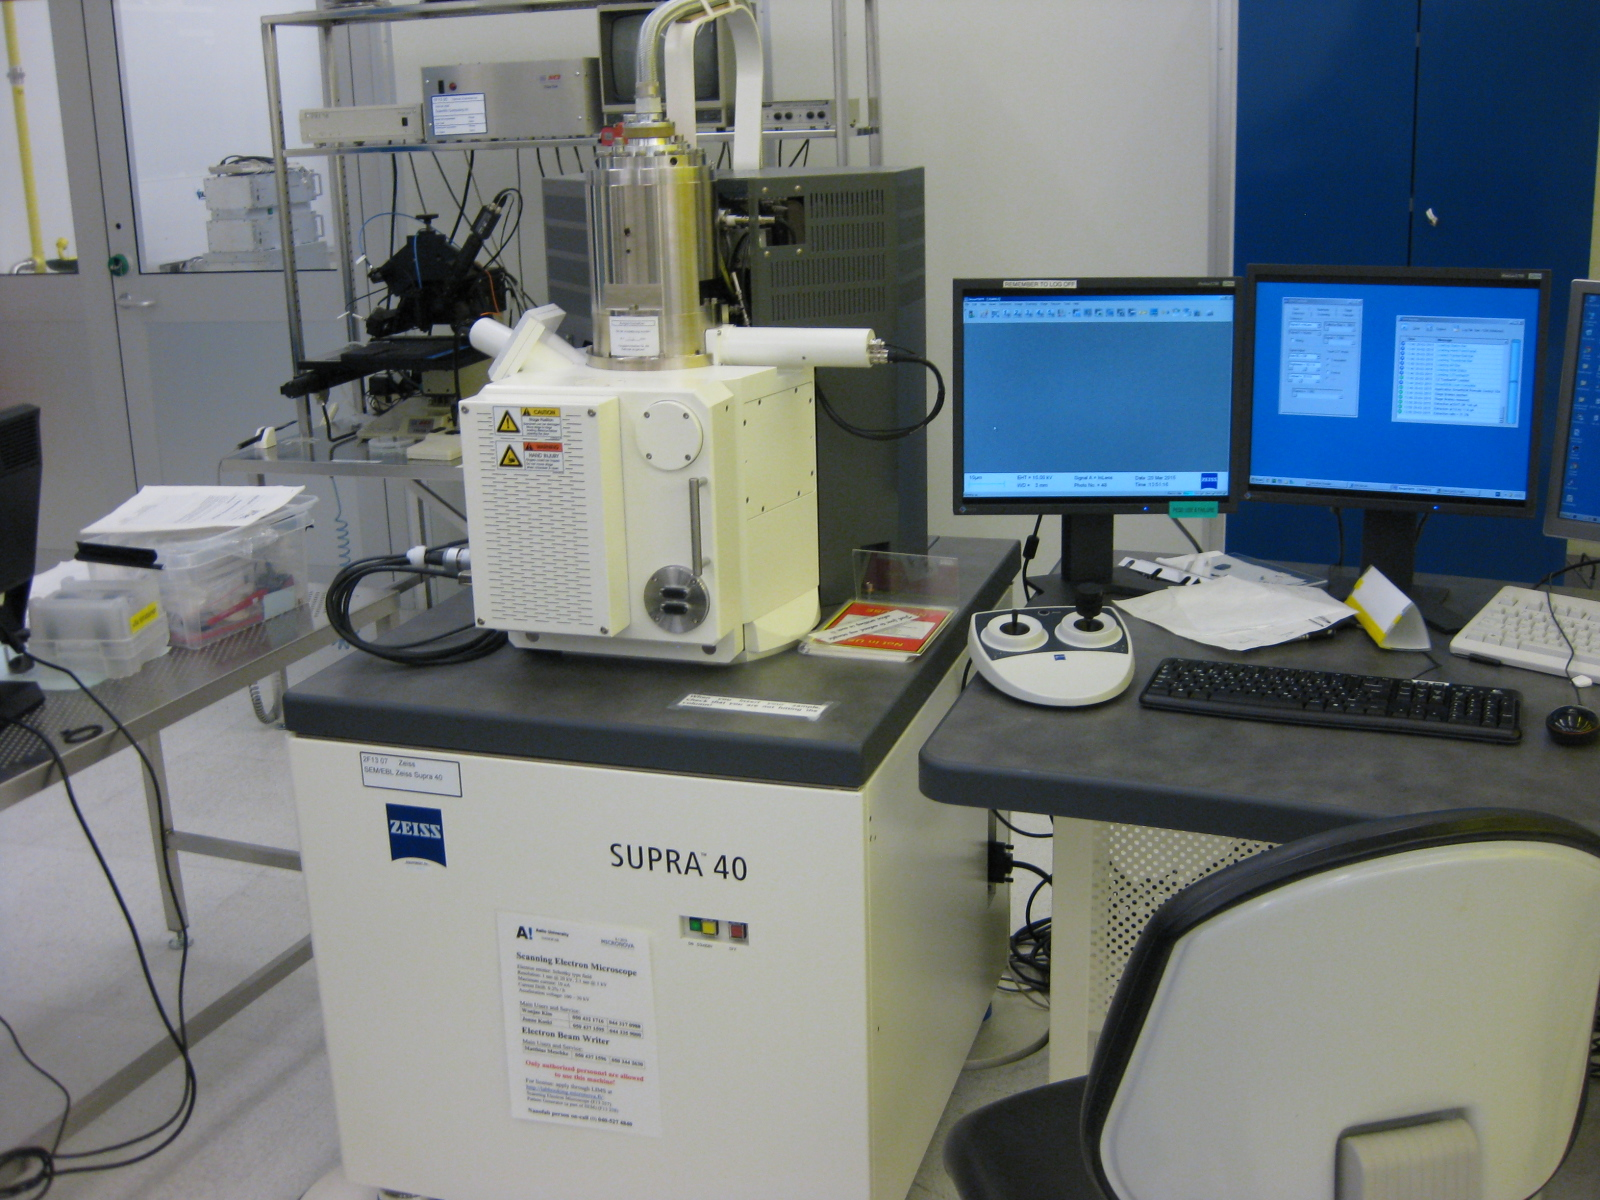
\includegraphics[width=200pt]{SEM.JPG}
                \caption{Scanning Electron Microscope used to observe the structures}
            \end{figure}
            
        \subsection{Observation of the samples}
            The SEM requires some adjustments in order to give us good images. The settings look very like optical settings : focus, stigmatism, aperture... To set them, we first choose a place where there is no samples, in order to avoid to charge them since we send electron within the matter. Of course, if there is nothing at all, it will be very difficult to set anything, so we choose a place with metal but which does not belong to a structure. Once the location chosen, we have to set the different parameters to get the best image possible. We align both focus and stigmation together by adjusting, and zooming when we have the optimal settings. The more we zoom in, the more tricky it becomes to get a good image. Then, while we consider that the image is good, which means precise enough and clear, we can start to observe the samples (Fig. \ref{SEMexemple}). We still have to pay attention not to charge them, so we try to observe fastly to avoid any problem. We do not need to observe each sample, we just take some pictures to check if the sample seems good in average. It is quite easy to detect if there has been a huge problem but the images only give an indication about the samples. Some samples seems bad and while we measure them, there are totally accurate whereas sometimes they seem quite good but the measurements show odd results. 
            
            \begin{figure}[H]
                \centering
                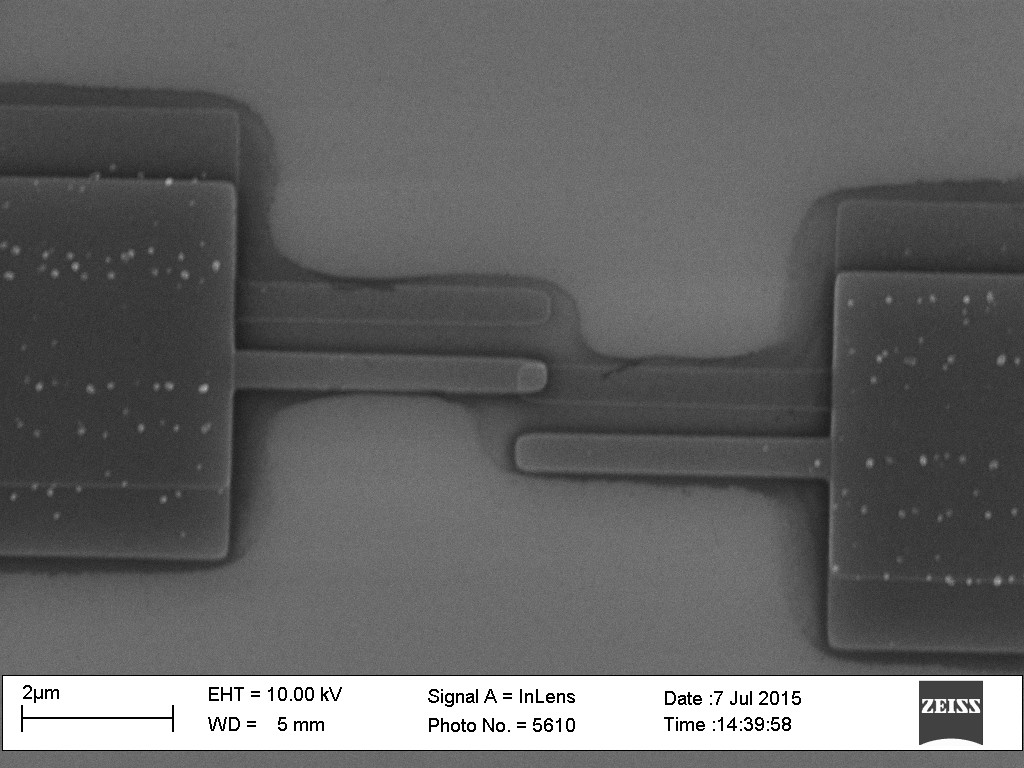
\includegraphics[width=300pt]{SEMexemple.jpg}
                \caption{SEM image of a sample}
                \label{SEMexemple}
            \end{figure}
            
            
            \section{Dilution cryostat}
            
            The cryostat is not a clean room device, though it is very useful for a low temperature laboratory. Since, I used it to cool down some samples we can consider it is part of the process to get some results and it is definitely an experimental device. First, I will talk about some theory to set the fridge up, then I will talk about the cooling down procedure we follow to reach 50mK.
            
            \subsection{Theory about Helium}
            %phase diagram He3 He4 -> mixture
            
            
            \subsection{Cooling down}
            The cooling down process in itself is quite long even if there is not much to do but waiting most of the time. The first thing to do, once the sample stage is in place is to put the bottom of the fridge in liquid nitrogen to start the cool down.
            %Pump, wait, pump, wait, pump...
            
            
            \subsection{Warming up}
            
            
            
